\documentclass{beamer}
\usepackage{amsmath, amssymb}
\usepackage{graphicx}
\usepackage{listings}
\usepackage{color}
\usepackage{subfig}
\usepackage{hyperref}
\usepackage{tcolorbox,fancyvrb,xcolor,tikz}
\tcbuselibrary{skins,breakable}

\newenvironment{VerbatimIN}
 {\VerbatimEnvironment
  \begin{tcolorbox}[
    breakable,
    colback=lightgray,
    spartan
  ]%
  \begin{Verbatim}}
 {\end{Verbatim}\end{tcolorbox}}

 \newenvironment{VerbatimOUT}
 {\VerbatimEnvironment
  \begin{tcolorbox}[
    breakable,
    spartan
  ]%
  \begin{Verbatim}}
 {\end{Verbatim}\end{tcolorbox}}

% R code formatting
\definecolor{codegreen}{rgb}{0,0.6,0}
\definecolor{codegray}{rgb}{0.5,0.5,0.5}
\definecolor{codepurple}{rgb}{0.58,0,0.82}
\definecolor{backcolour}{rgb}{0.95,0.95,0.92}
\lstdefinestyle{Rstyle}{
    backgroundcolor=\color{backcolour},
    commentstyle=\color{codegreen},
    keywordstyle=\color{magenta},
    numberstyle=\tiny\color{codegray},
    stringstyle=\color{codepurple},
    basicstyle=\ttfamily\footnotesize,
    breakatwhitespace=false,
    breaklines=true,
    captionpos=b,
    keepspaces=true,
    numbers=left,
    numbersep=5pt,
    showspaces=false,
    showstringspaces=false,
    showtabs=false,
    tabsize=2
}

\title{Mixed Effects Models - Week 12}
\subtitle{The Bayesian Linear Model}
\author{Marieke Wesselkamp\\Department of Biometry and Environmental Systems Analysis\\Albert-Ludwigs-University of Freiburg (Germany)}
\date{January 2025}

\begin{document}
\frame{\titlepage}

\begin{frame}
    \frametitle{Why Bayes?}
    \large
    \begin{itemize}
        \item Likelihood based models (GLM, ANOVA, t-test) do not address the question we are actually interested in:
        \item[] $P(hypothesis|data) \neq P(data|hypothesis)$
        \item We can include previous knowledge from preceeding research
        \item Bayesian algorithms are more robust
    \end{itemize}
\end{frame}

\begin{frame}
    \frametitle{What makes a Bayesian Model "Bayesian"?}
    \large
    \textbf{It consists of three parts:}
    \begin{itemize}
        \item The likelihood $p(y|\theta)$, which is the probability of the data given some hypothesis
        \item A prior assumption for every parameter from our hypothesis $p(\theta)$
        \item The posterior distribution $p(\theta|y)$, which is the probability of our hypothesis, given the data
    \end{itemize}
\end{frame}

\begin{frame}
    \frametitle{Concepts of Bayesian Statistics}
    \large
    The posterior is logically derived from the likelihood and prior distribution, and this logic follows Bayes' theorem, that is:
    \[
    p(\theta|y) = \frac{p(y|\theta) \cdot p(\theta)}{p(y)} = \frac{p(y|\theta) \cdot p(\theta)}{\int p(y|\theta) \cdot p(\theta) \cdot d\theta}
    \]
    \vspace{0.2cm}

    \textit{The posterior distribution summarizes the information from data and prior}
\end{frame}

\begin{frame}
    \frametitle{Bayes Theorem: Derivation}
    \begin{columns}
        \begin{column}{0.5\textwidth}
            The probability that two events occur, called the joint probability $\mathbf{P(A \cap B)}$, is the probability of $\mathbf{A, P(A)}$ times the probability of $\mathbf{B}$ given as $\mathbf{A}$ has occurred, $\mathbf{P(B|A)}$.
        \end{column}
        \begin{column}{0.5\textwidth}
            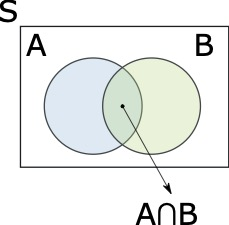
\includegraphics[width=\textwidth]{lectures/day_11_bayesian_lm/figures/joint_prob.jpg}
        \end{column}
    \end{columns}
\end{frame}

\begin{frame}
    \frametitle{Bayes Theorem: Derivation}
    \large
    The probability that two events occur, called the joint probability $P(A \cap B)$, is the probability of $A$, $P(A)$ times the probability of $B$ given $A$ has occurred, $P(B|A)$.
    \[
    P(A \cap B) = P(B|A) P(A)
    \]
    This is just as true as the other way around:
    \[
    P(A \cap B) = P(B|A) P(A) = P(A|B) P(B)
    \]
    Resolving the latter part gives us Bayes' Theorem:
    \[
    P(B|A) = \frac{P(A|B) \cdot P(B)}{P(A)}
    \]
\end{frame}

\begin{frame}
    \frametitle{Bayes Theorem: Example}
    \large
    We have a turtle population with 60\% female and 40\% male turtles. We know that of the female turtles, 10\% wear a transmitter and of the male 5\%. If we catch a turtle with a transmitter, what is the probability that it is female?
    \vspace{0.5cm}
    \[
    P(B|A) = \frac{P(A|B) \cdot P(B)}{P(A)}
    \]
    
\end{frame}

\begin{frame}
    \frametitle{Bayes Theorem: Example}
    \large

    \begin{itemize}
    \item \textbf{Probabilities of being male or female:}
    \begin{align*}
        P(\text{Female}) &= 0.6  \\
        P(\text{Male}) &= 0.4 
    \end{align*}

    \item \textbf{Conditional probabilities of wearing a transmitter:}
    \begin{align*}
        P(\text{Transmitter} \mid \text{Female}) &= 0.1  \\
        P(\text{Transmitter} \mid \text{Male}) &= 0.05 
    \end{align*}

    \item \textbf{What we want to find:}
    \begin{align*}
        P(\text{Female} \mid \text{Transmitter}) &= ?
    \end{align*}

    \item \textbf{But what is $P(\text{Transmitter})$ ?}
    \begin{align*}
        P(A) = \sum_i P(A \cap B_i)?
    \end{align*}
\end{itemize}
\end{frame}

\begin{frame}
    \frametitle{Bayes Theorem: Application}
    We can make use of this theorem by translating $A$ and $B$ into \textbf{data} $y$ and \textbf{model parameters} $\theta$.\\
    \[
    P(\theta|y) = \frac{P(y|\theta) \cdot P(\theta)}{P(y)}
    \]
    \vspace{0.2cm}
    
    \textit{The probability of our hypothesis GIVEN the data is the probability of the data given the hypothesis times the prior knowledge about the observations, standardized by the probability of the data.}
    \vspace{0.2cm}
    
    In terms of fitting a linear model, the hypothesis concerns the effect sizes. 
\end{frame}

\begin{frame}
    \frametitle{The Bayesian Linear Model}
    \begin{columns}
        \begin{column}{0.4\textwidth}
            A (fictious) relationship between nutrient concentration and plant biomass...
        \end{column}
        \begin{column}{0.6\textwidth}
            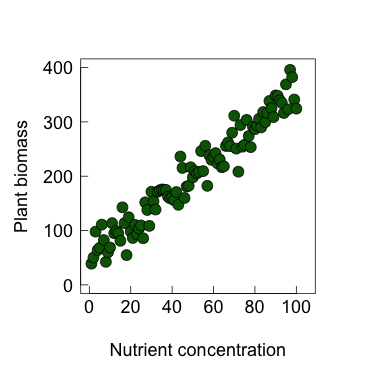
\includegraphics[width=\textwidth]{lectures/day_11_bayesian_lm/figures/unnamed-chunk-2-1.png}
        \end{column}
    \end{columns}
\end{frame}

\begin{frame}
    \frametitle{The Bayesian Linear Model}
    \begin{columns}
        \begin{column}{0.4\textwidth}
            ... described by this \textbf{model}:
            \[
            y = \beta_0 + \beta_1 \cdot x + \epsilon
            \]
            with the assumption that $\epsilon$ is \textit{iid}:
            \[
            \epsilon \sim N(0, \sigma^2)
            \]
        \end{column}
        \begin{column}{0.6\textwidth}
            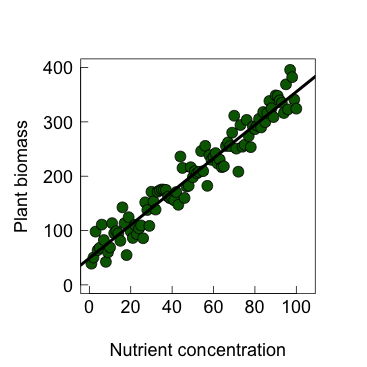
\includegraphics[width=\textwidth]{lectures/day_11_bayesian_lm/figures/unnamed-chunk-3-1.png}
        \end{column}
    \end{columns}
\end{frame}

\begin{frame}
    \frametitle{The Bayesian Linear Model}
    \begin{columns}
        \begin{column}{0.4\textwidth}
            Can also be formalized through the parametric
            \textbf{Likelihood}-assumption:
            \[
            y \sim Normal(\mu, \sigma_\epsilon^2)
            \]
            With additional \textbf{Parameters}
            \[
            \mu = \beta_0 + \beta_1 \cdot x
            \]
            \textit{In the Bayesian approach, $\beta_0$, $\beta_1$ and $\sigma_\epsilon$ are also considered random variables from prior probability distributions}
        \end{column}
        \begin{column}{0.6\textwidth}
            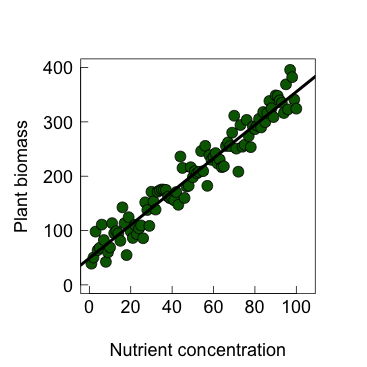
\includegraphics[width=\textwidth]{lectures/day_11_bayesian_lm/figures/unnamed-chunk-4-1.png}
        \end{column}
    \end{columns}
\end{frame}

\begin{frame}
    \frametitle{The Bayesian Linear Model}
    \begin{columns}
        \begin{column}{0.4\textwidth}
            The data generating process determines the \textcolor{red}{Likelihood}-function:
            \[
            y \sim Normal(\mu, \sigma_\epsilon^2)
            \]
            Previous knowledge determines the choice of Prior distributions for \textcolor{red}{Parameters}:
            \[
            \mu = \beta_0 + \beta_1 \cdot x
            \]
        \end{column}
        \begin{column}{0.6\textwidth}
            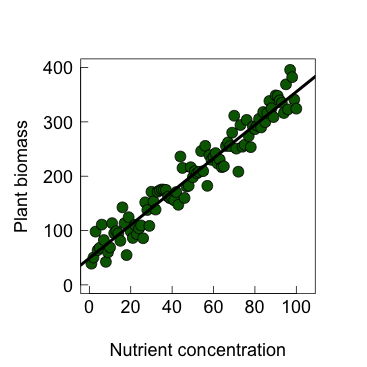
\includegraphics[width=\textwidth]{lectures/day_11_bayesian_lm/figures/unnamed-chunk-5-1.png}
        \end{column}
    \end{columns}
\end{frame}

\begin{frame}
    \frametitle{The Bayesian Linear Model}
    \begin{columns}
        \begin{column}{0.6\textwidth}
            The data generating process determines the \textcolor{red}{Likelihood}-function:\\
            \[
            y \sim Normal(\mu, \sigma_\epsilon^2)
            \]
            \[
            \mu = \beta_0 + \beta_1 \cdot x
            \] 
            Previous knowledge determines the choice of Prior distributions for \textcolor{red}{Parameters}:
            \begin{align*}
                \beta_0 \sim Normal(200,50) \quad \textcolor{red}{Prior} \\
                \beta_1 \sim Normal(5,1) \quad \textcolor{red}{Prior} \\
                \sigma_\epsilon \sim Uniform(0,30) \quad \textcolor{red}{Prior}
            \end{align*}
        \end{column}
        \begin{column}{0.4\textwidth}
            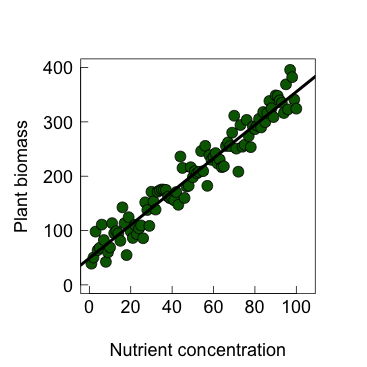
\includegraphics[width=\textwidth]{lectures/day_11_bayesian_lm/figures/unnamed-chunk-5-1.png}
        \end{column}
    \end{columns}
\end{frame}

\begin{frame}
    \frametitle{Sampling from the Posterior}
    We have one issue in the definition of Bayes' Theorem:
    \[
    P(\theta|y) = \frac{P(y|\theta) \cdot P(\theta)}{P(y)}
    \]
    \vspace{0.2cm}

    \textit{The probability of our hypothesis GIVEN the data is the probability of the data given the hypothesis times the prior knowledge of the observations, standardized by the probability of the data.}
    \vspace{0.2cm}

    \textbf{The problem lies in P(y)!}
\end{frame}

\begin{frame}
    \frametitle{Sampling from the Posterior}
    Why is P(y) horrible?:
    \[
    P(y) = \sum_\theta P(y|\theta) P(\theta)
    \]
    \vspace{0.2cm}

    \textit{When $\theta$ consists of more than two options, this divisor gets very ugly quite fast. Often we are not able to calculate it.}
    \vspace{0.2cm}

    \textbf{We get rid of it by sampling from the posterior distribution} $\mathbf{P(\theta|y)}$
\end{frame}

\begin{frame}
    \frametitle{Sampling from the Posterior}
    \large
    We can say that:
    \[
    1.\quad P(\theta|y) \propto P(y|\theta) \times P(\theta)
    \]
    \[
    2.\quad \frac{P(\theta_1|y)}{P(\theta_2|y)} = \frac{P(y|\theta_1) \times P(\theta_1)}{P(y|\theta_2) \times P(\theta_2)} = \alpha
    \]
    \vspace{0.2cm}
    
    These properties we use to sample from the posterior distribution with numerical sampling algorithms.
\end{frame}

\begin{frame}
    \frametitle{Sampling Algorithms}
    \Large
    \textbf{Popular Sampling Algorithms:}
    \vspace{0.2cm}
    
    \begin{itemize}
        \item Rejection sampling
        \item \textbf{Markov-Chain Monte Carlo (MCMC)}
        \item Sequential Monte Carlo
    \end{itemize}
\end{frame}

\begin{frame}
    \frametitle{Metropolis-Hastings MCMC}
    The Metropolis-Hastings MCMC allows sampling from complex distributions, where direct sampling is impractical.
    \begin{enumerate}
        \item Pick random start values for the parameters $\theta_1$
        \item Based on a proposal function (e.g. $Normal(\theta_1, \sigma)$, propose a new value: $\theta_2$
        \item Compute: \[\alpha = \frac{P(\theta_2|y)}{P(\theta_2|y)}\]
        \item The posterior ratio $\alpha$ determines if the new values $\theta_2$ will be accepted:
        \item[] if $\alpha > 1$: accept $\theta_2$
        \item[] if $\alpha < 1$: accept $\theta_2$ \textbf{sometimes}, otherwise reject and accept $\theta_1$
        \item Repeat for many iterations
    \end{enumerate}
\end{frame}

\begin{frame}
    \frametitle{Metropolis-Hastings MCMC}
    \begin{center}
        \large\textbf{Let's fit a regression to this artificial data set using Bayes' Theorem}\\
        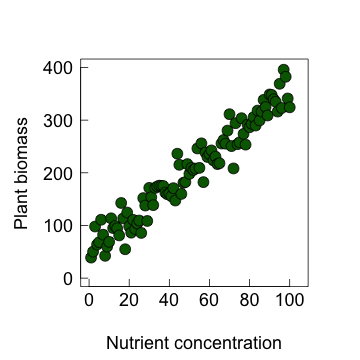
\includegraphics[width=0.6\textwidth]{lectures/day_11_bayesian_lm/figures/unnamed-chunk-7-1.png}
    \end{center}
\end{frame}

\begin{frame}
    \frametitle{Metropolis-Hastings MCMC}
    \large
    1. Define the statistical model and the likelihood function:\vspace{0.3cm}
    
    $y \sim Normal(\mu, \sigma_\epsilon^2)$  \textcolor{red}{Likelihood} \\
    $\mu = \beta_0 + \beta_1 \cdot x$  \textcolor{red}{Parameters}

    \begin{columns}
        \begin{column}{0.4\textwidth}
            2. Plot the \textbf{log-likelihood of the data for varying values of} $\mathbf{\beta_1}$:
        \end{column}
        \begin{column}{0.6\textwidth}
            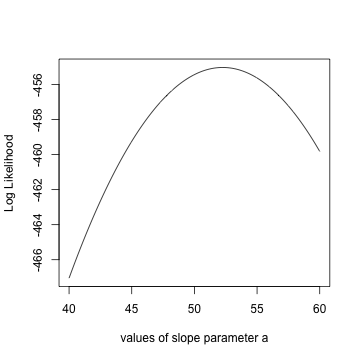
\includegraphics[width=0.8\textwidth]{lectures/day_11_bayesian_lm/figures/unnamed-chunk-9-1.png}
        \end{column}
    \end{columns}
\end{frame}

\begin{frame}
    \frametitle{Metropolis-Hastings MCMC}
    \large
    \begin{columns}
        \begin{column}{0.4\textwidth}
            3. Define the priors as \textbf{log-densities}:
        \end{column}
        \begin{column}{0.6\textwidth}
            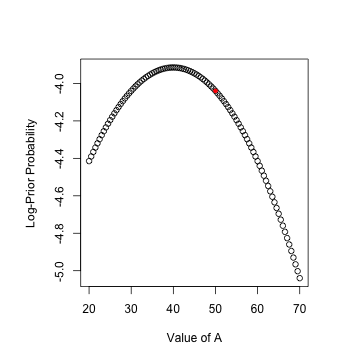
\includegraphics[width=0.8\textwidth]{lectures/day_11_bayesian_lm/figures/unnamed-chunk-10-1.png}
        \end{column}
    \end{columns}
        4. Compute the Posterior:
        \begin{align}
    \log(p(\beta_0, \beta_1, \sigma \mid y)) &= 
    \log(p(y \mid \beta_0, \beta_1, \sigma)) \nonumber \\
    &\quad + \log(p(\beta_0)) + \log(p(\beta_1)) + \log(p(\sigma))
\end{align}
\end{frame}

\begin{frame}[fragile]
    \frametitle{Metropolis-Hastings MCMC in R}
    1. Pick random start values for the parameters $\theta_1$
    \scriptsize
    \begin{VerbatimIN}[numbers=left,numbersep=6pt]
startvalue = c(50, 3, 10)
    \end{VerbatimIN}
    \normalsize
    2. Based on a proposal function (e.g. $Normal(\theta_1, \sigma)$), propose a new value $\theta_2$
    \scriptsize
    \begin{VerbatimIN}[numbers=left,numbersep=6pt]
proposal = rnorm(3, mean = startvalue, sd=c(0.5, 0.1, 0.5))
    \end{VerbatimIN}
    \normalsize
    3. Compute
    \[
    \alpha = \frac{P(\theta_2|y)}{P(\theta_1|y)}
    \]
    \scriptsize
    \begin{VerbatimIN}[numbers=left,numbersep=6pt]
probab = exp(posterior(proposal) - posterior(startvalue))
    \end{VerbatimIN}
\end{frame}

\begin{frame}[fragile]
    \frametitle{Metropolis-Hastings MCMC in R}
    4. Run the Metropolis MCMC for any start-value for parameters.\\
    The posterior ratio $\alpha$ determines, wether the new values $\theta_2$ are going to be accepted:\vspace{0.2cm}
    
    if $\alpha > 1$: accept $\theta_2$\\
    if $\alpha < 1$: accept $\theta_2$ sometimes, otherwise keep $\theta_1$
    \vspace{0.2cm}

    \scriptsize
    \begin{VerbatimIN}[numbers=left,numbersep=6pt]
if (runif(1) < probab){
      # accept ...
    }
    \end{VerbatimIN}
    \normalsize
    Repeat for $i$ iterations
\end{frame}

\begin{frame}
    \frametitle{Metropolis-Hastings MCMC in R}
    After $i$ iterations, our parameter samples (left) and the according posterior distributions (right) for this example look like this (using the R coda package):
    \begin{center}
    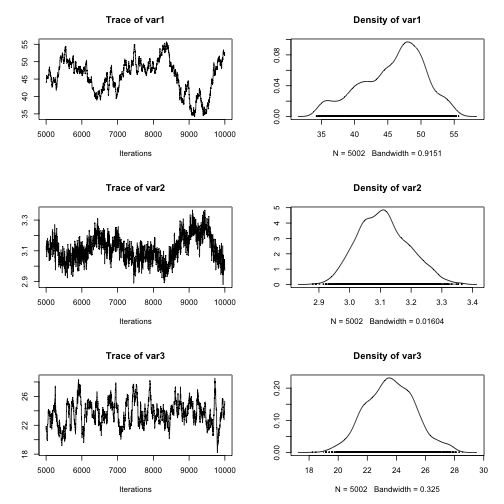
\includegraphics[width=0.65\textwidth]{lectures/day_11_bayesian_lm/figures/unnamed-chunk-17-1.png}        
    \end{center}
\end{frame}

\begin{frame}[fragile]
    \frametitle{Metropolis-Hastings MCMC in R}
    5. Compare MCMC estimates and LM estimates
    \begin{columns}
        \begin{column}{0.5\textwidth}
            \tiny
            \begin{VerbatimIN}[numbers=left,numbersep=6pt]
summary(result)
            \end{VerbatimIN}
            \begin{VerbatimOUT}[numbers=left,numbersep=6pt]
Iterations = 5000:10001
Thinning interval = 1 
Number of chains = 1 
Sample size per chain = 5002 

1. Empirical mean and standard deviation 
for each variable,plus standard error 
of the mean:

      Mean      SD Naive SE Time-series SE
[1,] 45.86 4.74233 0.067053        1.95165
[2,]  3.11 0.08311 0.001175        0.02079
[3,] 23.60 1.68435 0.023816        0.24290

2. Quantiles for each variable:

       2.5%   25%    50%    75%  97.5%
var1 35.399 42.49 46.804 49.316 53.992
var2  2.964  3.05  3.105  3.166  3.279
var3 20.404 22.40 23.595 24.764 27.060
            \end{VerbatimOUT}
        \end{column}
        \begin{column}{0.6\textwidth}
            \tiny
            \begin{VerbatimIN}[numbers=left,numbersep=6pt]
summary(lm(y ~ x))
            \end{VerbatimIN}
            \begin{VerbatimOUT}[numbers=left,numbersep=6pt]
Call:
lm(formula = y ~ x)

Residuals:
    Min      1Q  Median      3Q     Max 
-61.339 -13.809  -0.866  16.212  52.372 

Coefficients:
            Estimate Std. Error t value Pr(>|t|)    
(Intercept)  49.0899     4.6072   10.65   <2e-16 ***
x             3.0628     0.0792   38.67   <2e-16 ***
---
Signif. codes:  0 '***' 0.001 '**' 0.01 '*' 
                0.05 '.' 0.1 ' ' 1
Residual standard error: 
22.86 on 98 degrees of freedom
Multiple R-squared:  
0.9385,    Adjusted R-squared:  0.9379 
F-statistic:  
1495 on 1 and 98 DF,  p-value: < 2.2e-16
            \end{VerbatimOUT}
        \end{column}
    \end{columns}
\end{frame}

\begin{frame}[fragile]
    \frametitle{Metropolis-Hastings MCMC in R}
    6. Run a second chain and combine \vspace{0.4cm}
    
    \begin{columns}
        \begin{column}{0.45\textwidth}
            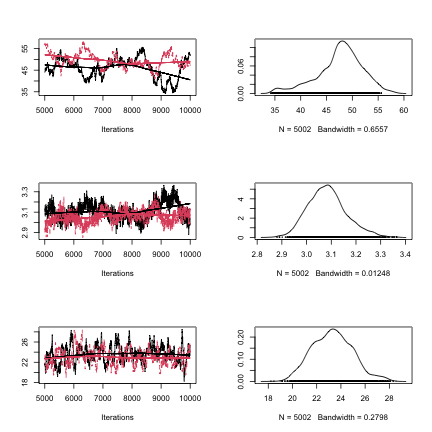
\includegraphics[width=\textwidth]{lectures/day_11_bayesian_lm/figures/unnamed-chunk-20-1.png}
        \end{column}
        \begin{column}{0.55\textwidth}
            Check for convergence:\\
            The Gelman-Rubin measure or \textit{scale reduction factor} $\hat{R}$
            \scriptsize
            \begin{VerbatimIN}[numbers=left,numbersep=6pt]
coda::gelman.diag(combinedchains)
            \end{VerbatimIN}
            \begin{VerbatimOUT}[numbers=left,numbersep=6pt]
Potential scale reduction factors:

     Point est. Upper C.I.
[1,]       1.41       2.38
[2,]       1.27       1.90
[3,]       1.06       1.24

Multivariate psrf

1.25
            \end{VerbatimOUT}
        \end{column}
    \end{columns}
\end{frame}

\begin{frame}
    \frametitle{}
    \large
    There is a range of probabilistic programming languages that allow for very flexible implementation of complex hierarchical Bayesian models and provide large libraries of distributions.\vspace{0.3cm}

    Old School: WinBUGS \vspace{0.2cm}
    
    Modern: JAGS, Stan, Nimble \vspace{0.3cm}
    
    \textit{The modern languages are also accessible through R!}
\end{frame}

\begin{frame}[fragile]
    \frametitle{Model Example in JAGS}
    \scriptsize
    \begin{VerbatimIN}[numbers=left,numbersep=6pt]
library(rjags)
library(R2jags)

jagsmodel <- textConnection('
                          model {
                            # prior
                            beta0 ~ dnorm(50, 20)
                            beta1 ~ dnorm(0, 20)
                            tau ~ dunif(0, 30)
                            sigma <- 1/sqrt(tau)

                            # likelihood
                            for (i in 1:N){
                              mu[i] <- beta0 + beta1*x[i]
                              y[i] ~ dnorm(mu[i], tau)
                            }
                            }
                            ')
    \end{VerbatimIN}
\end{frame}

\begin{frame}[fragile]
    \frametitle{Model Example in JAGS}
    \scriptsize
    \begin{VerbatimIN}[numbers=left,numbersep=6pt]
data <-  list(x = x, y = y, N = length(x))
params <-  c("beta0", "beta1", "sigma")

jagsModel <- jags.model( file= jagsmodel , data=data, n.chains = 3, 
                         n.adapt= 500, quiet=TRUE)
results <- coda.samples( jagsModel , variable.names=params,
                         n.iter=5000)
    \end{VerbatimIN}
\end{frame}

\begin{frame}[fragile]
    \frametitle{Model Example in JAGS}
    \scriptsize
    \begin{VerbatimIN}[numbers=left,numbersep=6pt]
plot(results)
    \end{VerbatimIN}
    \begin{center}
        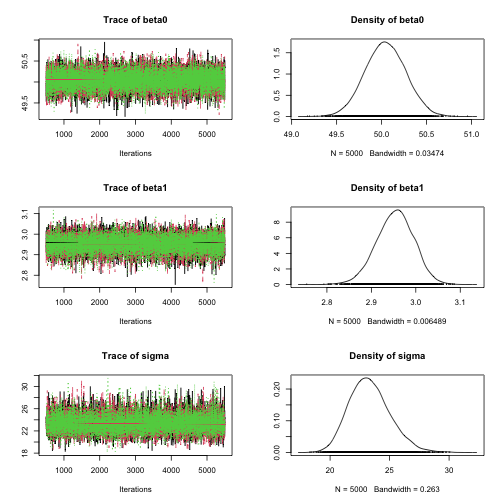
\includegraphics[width=0.65\textwidth]{lectures/day_11_bayesian_lm/figures/unnamed-chunk-23-1.png}
    \end{center}
\end{frame}

\begin{frame}[fragile]
    Estimates from JAGS' Gibbs sampling have a larger signal-to-noise ratio than those from the Metropolis-Hastings MCMC algorithm...
    \scriptsize
    \begin{VerbatimIN}[numbers=left,numbersep=6pt]
summary(results)
    \end{VerbatimIN}
    \begin{VerbatimOUT}[numbers=left,numbersep=6pt]
Iterations = 501:5500
Thinning interval = 1 
Number of chains = 3 
Sample size per chain = 5000 

1. Empirical mean and standard deviation for each variable,
   plus standard error of the mean:
        Mean      SD  Naive SE Time-series SE
beta0 50.043 0.22427 0.0018311      0.0018306
beta1  2.953 0.04189 0.0003421      0.0003944
sigma 23.334 1.73086 0.0141324      0.0168952

2. Quantiles for each variable:
        2.5%    25%    50%    75%  97.5%
beta0 49.604 49.891 50.042 50.195 50.480
beta1  2.869  2.926  2.955  2.982  3.032
sigma 20.327 22.122 23.213 24.397 27.030
    \end{VerbatimOUT}
\end{frame}

\begin{frame}
\frametitle{Recapitulation Week 11}
    Key concepts covered today:
    \begin{itemize}
        \item Bayes' Theorem
        \item Components of the Bayesian Linear Model:
        \item[] \textbf{Likelihood, Priors and Posteriors}
        \item Bayesian tools: Sampling algorithms
        \item Model calibration on foot (MH MCMC) and via JAGS
    \end{itemize}
    \vspace{0.2cm}

    Today's exercises: Bayes and MH MCMC sampling
\end{frame}

\begin{frame}
    \frametitle{Further Readings}
    \Large
    \begin{enumerate}
        \item \href{https://www.biom.uni-freiburg.de/mitarbeiter/dormann/stats-gna.pdf}{Bayesscher Anhang zu "Parametrische Statistik" (Dormann 2019)}
        \item \href{https://florianhartig.github.io/LearningBayes/}{Introduction to Bayesian Statistics with R (Hartig 2024)}
        \item \href{https://michael-franke.github.io/intro-data-analysis/}{An Introduction to Data Analysis (Franke 2023)}
    \end{enumerate}

\end{frame}



    
\end{document}